\subsection{Model}\label{sec:cloud:crowdsourcing:model}

In our model, schematically depicted in \reffig{fig:sec:cloud:crowdsourcing:model:model}, we consider a crowdsourcing  platform employing \(\numberOfWorkers\) workers.
The time between two campaigns being submitted is given by the random variable \(\campaignIAT\)
Each campaign consists of a number of tasks, distributed according to the random variable \(\campaignSize\).
We assume that each task is then completed by one of the \(\numberOfWorkers\) workers in order of arrival.
The time required for completion is given by the random variable \(\taskDuration\).

\begin{figure}
  \centering
  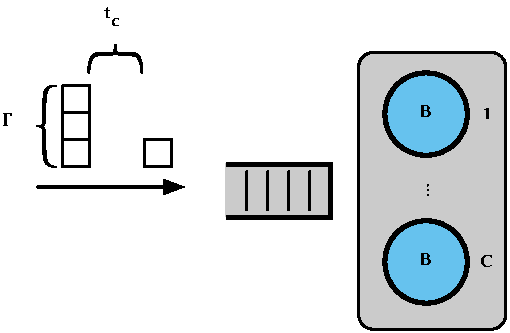
\includegraphics{cloud/crowdsourcing/model/figures/model}
  \caption{Considered crowdsourcing platform model.}
  \label{fig:sec:cloud:crowdsourcing:model:model}
\end{figure}

From this model we derive two metrics in order to evaluate the performance of the crowdsourcing platform.
First, we consider the utilisation \(\workerUtilization\) for all workers.
This can be interpreted as a measure of earning potential for workers on the platform and should be maximized in order to keep current workers and attract new ones. 
Furthermore, we seek to obtain the mean task pre-processing delay \(\preTaskProcessingDelay\), i.e., the time occurring before a worker begins to work on a task.
This measure is relevant for the employer and should be minimised.
We use the mean task pre-processing delay \(\preTaskProcessingDelay\) instead of the average completion time of the campaigns, as the completion time also depends on the task length, which is under control of the employer and not the platform operator.

In this section we first introduce an analytical model, which will be used to validate the simulation model discussed thereafter.
Finally, a comparative validation of the analytical and simulative model is performed.

\subsubsection*{Analytical Consideration}

First, in order to provide exact results, we consider the crowdsourcing platform as a \(M^{[\campaignSize]}/M/\numberOfWorkers-\infty\) model.
Here, we assume both the campaign inter-arrival time \(\campaignIAT\) as well as the time to complete a task \(\taskDuration\) to be exponentially distributed with mean \(E[\campaignIAT] = \frac{1}{\lambda}\) and \(E[B] = \nicefrac{1}{\mu}\), due to the large number of employers submitting tasks and the large number of workers completing them.
Furthermore, we model the number of tasks per campaign \(\campaignSize\) using a geometric distribution with mean \(E[\campaignSize] = \nicefrac{1}{p}\).

This model is well studied and state probabilities are provided in \cite{Kleinrock1975} or \cite{TranGia1982} for the case of a loss system.

Based on these state probabilities, we obtain the mean utilisation \workerUtilization per service unit as
\[
\workerUtilization = \sum_{i=0}^{\kappa} \min(i, c) x(i) = \frac{\lambda E[\campaignSize]}{c\mu}. 
\]
This metric can be used to quantify the income of a worker, as a higher utilisation results in a higher income.

Next, we obtain the mean queue length \(\Omega\) of the system as
\[
	\Omega = \sum_{i = c}^\kappa (i - c) x(i).
\]
Now, we consider the mean task pre-processing delay \preTaskProcessingDelay and with Little's theorem applied to the systems queue, we get
\[\lambda E[\campaignSize] \preTaskProcessingDelay = \Omega.\]

We solve for task the pre-processing delay \preTaskProcessingDelay~and obtain
\[\preTaskProcessingDelay = \frac{\Omega}{\lambda E[\campaignSize]}.\]

\subsubsection*{Simulation}

In order to allow for a larger variety of campaign inter-arrival time distributions \(\campaignIAT\), we implement a discrete event simulation using the OMNet++ simulation framework\footnote{\url{http://www.omnetpp.org/}, \accessed}.
We augment the framework with support for bulk arrivals and support of empiric distributions taken from measurements described in \refsec{sec:cloud:crowdsourcing:measurements}.
Similar, to the queueing model introduced in this section, we consider campaign inter-arrivals according to a distribution \(\campaignIAT\) and a campaign size of \(\campaignSize\) tasks.
Task length is given by a distribution \(\taskDuration\) and tasks are stored in an unbounded queue before being sent to service to the \(\numberOfWorkers\) available workers.
During simulation, we record the mean utilisation \(\workerUtilization\) as well as the mean task pre-processing delay \(\preTaskProcessingDelay\).

\subsubsection*{Validation}

In this section, we validate the simulative model by comparing the metrics utilisation \(\workerUtilization\) and task pre-processing delay \(\preTaskProcessingDelay\) for a representative parameter set with those obtained from the analytic model.
We consider exponential campaign inter-arrival times \(\campaignIAT\) with a campaign rate of \SI{4}{\per\hour} campaigns, and a campaign size \campaignSize geometrically distributed with a mean of \(100\) tasks per campaign.
For the task length \taskDuration, we consider a set of suitable values, to accommodate for different task types, between \SIrange{60}{300}{\second} per task.
In both simulation and analytical model, we consider between \(5\) and \(50\) workers.

\begin{figure*}
	\centering
	\begin{subfigure}{\columnwidth}
		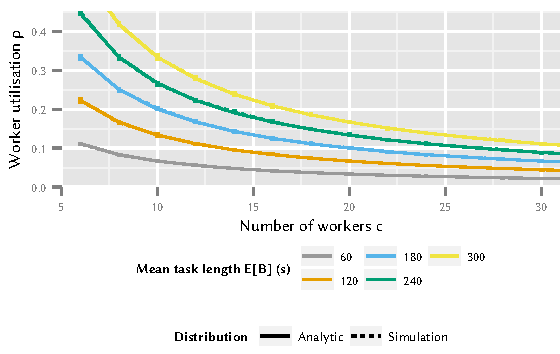
\includegraphics{cloud/crowdsourcing/model/figures/comparison_utilization}
		\caption{Utilisation \workerUtilization}
		\label{fig:cloud:crowdsourcing:validation:model:utilization}
	\end{subfigure}

	\begin{subfigure}{\columnwidth}
		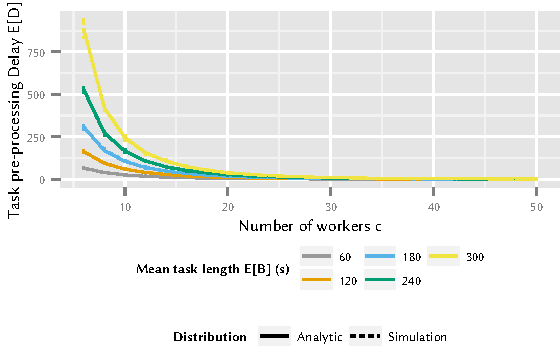
\includegraphics{cloud/crowdsourcing/model/figures/comparison_task_delay}
		\caption{Mean task pre-processing delay \preTaskProcessingDelay}
		\label{fig:cloud:crowdsourcing:validation:model:task_delay}
	\end{subfigure}
	\caption{Validation of simulation with analytic model.}
	\label{fig:cloud:crowdsourcing:validation:model}
\end{figure*}

Results are shown in \reffig{fig:cloud:crowdsourcing:validation:model}.
Simulative respective analytical results are shown by different line types.
However, due to the good fit of the analytic and simulative model, the line showing the simulative results completely covers the analytic results.
For the simulation we give \SI{95}{percent} confidence intervals based on \(10\) replications.
In this, and all following figures, confidence intervals are given as error bars.
For each simulation we consider a simulation duration of \SI{1500}{\hour} hours and accommodate for a transient phase of \SI{150}{\hour} hours.
We observe that for both the utilisation \workerUtilization and mean task pre-processing delays \preTaskProcessingDelay, the analytical results are well within the confidence intervals.